\documentclass[12pt]{beamer}
\usepackage{verbatim}
\usepackage{ifthen}

\usepackage{tikz}
\usetikzlibrary{arrows, positioning}
\usepackage{pgfplots}
\usepackage{onimage}
\usepackage{url}

\newcommand{\bigpic}[1]{
\begin{center}
\includegraphics[width=\textwidth, height=0.8\textheight, keepaspectratio]{#1}
\end{center}
}
 
% Specify theme
\usetheme{UnofficialUChicago}

% \setbeamertemplate{footline}[frame number]{} % Uncomment this line if you dont want the footer on each slide

%===============================================================%
% 				BEGIN YOUR PRESENTATION HERE					%
%===============================================================% 
 
% Title and author information
\title[RTI Models]{
Data-driven modeling of the low Atwood single mode Rayleigh-Taylor instability
}
\author{Maxwell Hutchinson}
\institute[UofC]{University of Chicago}
\date{\today}
  

%===============================================================%
\begin{document}
%===============================================================%

\newcommand{\pder}[2] {\frac{\partial #1}{\partial #2}}
\newcommand{\ppder}[2] {\frac{\partial^2 #1}{\partial #2^2}}
\newcommand{\der}[2] {\frac{d #1}{d #2}}
\newcommand{\dder}[2] {\frac{d^2 #1}{d #2^2}}
 
\maketitle

\begin{frame}{Outline}
\begin{enumerate}
  \item Background: Rayleigh-Taylor instability
  \item Motivation: understanding re-acceleration during nonlinear RT
  \item Hypothesis: buoyancy-drag model with viscosity
  \item Experiment: do direct numerical simulations match experiments?
  \item Experiment: does the model match direct numerical simulations?
  \item Results: yes and yes*
  \item Conclusions: viscosity, absent in other models, is important
\end{enumerate}

\end{frame}

%===============================================================%
\section{Background}
%===============================================================%

\begin{frame}{Rayleigh-Taylor Instability (RTI)}
\begin{columns}
\column{0.65\textwidth}
\begin{itemize}
\item[] The RTI occurs when pressure and density gradients oppose:
$$ (\mathbf{\nabla} p) \cdot (\mathbf{\nabla} \rho) < 0 $$
\end{itemize}
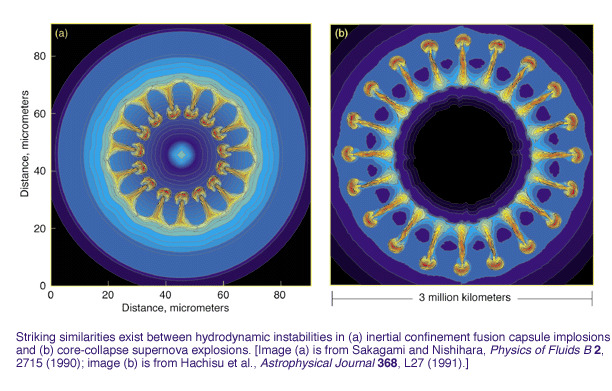
\includegraphics[width=\columnwidth]{graphics/icf}
\column{0.35\textwidth}
Soap left overnight\footnote{flowviz.tumblr.com}
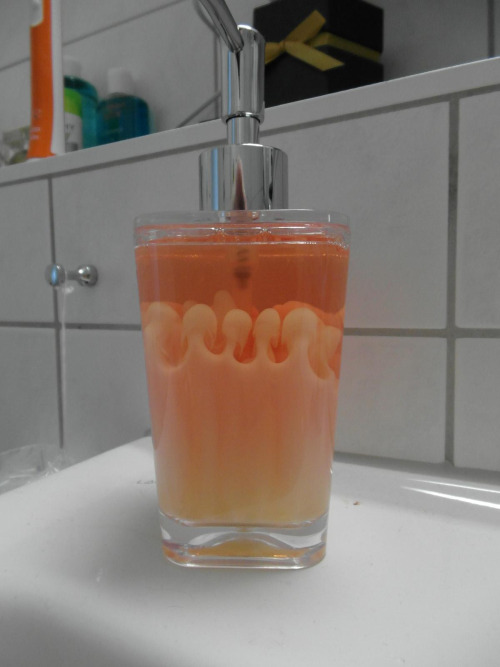
\includegraphics[width=\columnwidth]{graphics/soap}
\end{columns}
\end{frame}

\begin{frame}{Single mode low-Atwood Rayleigh-Taylor Instability}
\begin{columns}[c]

\column{0.65\textwidth}
\begin{block}{Approximations}
\begin{itemize}
	\item Boussinesq (low-Atwood): $A =(\rho_h-\rho_l) / (\rho_h+\rho_l) << 1$
  \item Uniform parameters: $\nu_l = \nu_h$
  \item Miscible: $D$ or $\alpha > 0$
  \item Incompressible: $\nabla \cdot \mathbf{u} = 0$
\end{itemize}
\end{block}

\begin{exampleblock}{Physical analogs}
\begin{itemize}
  \item Warm and cold water
  \item Salt and fresh water
\end{itemize}
\end{exampleblock}

\column{0.35\textwidth}
\resizebox{!}{0.9\textheight}{\tikzset{
  laser beam action/.style={
    line width=\pgflinewidth+.4pt,draw opacity=.1,draw=#1,
  },
  laser beam recurs/.code 2 args={%
    \pgfmathtruncatemacro{\level}{#1-1}%
    \ifthenelse{\equal{\level}{0}}%
    {\tikzset{preaction={laser beam action=#2}}}%
    {\tikzset{preaction={laser beam action=#2,laser beam recurs={\level}{#2}}}}
  },
  laser beam/.style={preaction={laser beam recurs={10}{#1}},draw opacity=1,draw=#1},
}

\begin{tikzpicture}[node distance=1cm, auto,]
%\draw[help lines, thick] (0,0) grid (8,16);
\draw (2,3) -- (2,13) -- (6,13) -- (6,3) -- cycle;
\draw[dashed] (2,8) -- (6,8);
\draw[laser beam=black] (2,8) to[out=85,  in=95,  distance=3.35cm] (3,8);
\draw[laser beam=black] (3,8) to[out=-85, in=-95, distance=3.35cm] (4,8);
\draw[laser beam=black] (4,8) to[out=85,  in=95,  distance=3.35cm] (5,8);
\draw[laser beam=black] (5,8) to[out=-85, in=-95, distance=3.35cm] (6,8);

\draw[white, fill=white] (1.5,7) rectangle (1.98,9);
\draw[white, fill=white] (6.02,7) rectangle (6.5,9);

\draw[dotted] (6,10.5) -- (2,10.5);
\draw[dotted] (6,5.5) -- (2,5.5);
\node[blue] at (4,12) {Heavy: $\rho_h$};
\node[red] at (4,4) {Light: $\rho_l$};
\draw[ultra thick, ->] (6.5,11) node[above] {g} -- (6.5,5);
\draw (2,13.1) edge[<->] node[above] {L} (6,13.1);
\draw (2,5.4) edge[<->] node[below] {$\lambda$} (4,5.4);
\draw (2,11) edge[<->] node[above] {$d$} (3,11);
\draw (2.88,8.2) edge[<->] node[above right] {$\delta$} (3.08,8.2);
\draw (1.8,8) edge[<->] node[left] {$h_b$} (1.8,10.5);
\draw (1.8,8) edge[<->] node[left] {$h_s$} (1.8,5.5);
\end{tikzpicture}

}
\end{columns}
\end{frame}

\begin{frame}{Governing equations}
\begin{exampleblock}{}
\begin{columns}
\begin{column}{0.5\linewidth}
\begin{itemize}
\item $\mathbf{u}$ is flow velocity
\item $\nu$ is kinematic viscosity
\end{itemize}
\end{column}
\begin{column}{0.5\linewidth}
\begin{itemize}
\item $\phi$ is active scalar
\item $D$ is diffusivity
\end{itemize}
\end{column}
\end{columns}
\end{exampleblock}
\begin{block}{Incompressible Navier-Stokes with active scalar}
\vspace{-20pt}
\begin{align*}
\der{\mathbf{u}}{t} &= \mathbf{u} \nabla \mathbf{u} - \nabla p - \nu \nabla^2 \mathbf{u} + A \mathbf{g} \phi  && \text{Momentum} \\
0 &= \nabla \cdot \mathbf{u} && \text{Incompressibility} \\ 
\der{\phi}{t} &= \mathbf{u} \nabla \phi - D \nabla^2 \phi && \text{Advection-diffusion} \\
\mathbf{u} &= \left. 0 \right|_{\partial \Omega}, \quad \quad \mathbf{n} \cdot \nabla \phi = \left. 0 \right|_{\partial \Omega}&& \text{Walls}
\end{align*}
\end{block}
\end{frame}

\begin{frame}
\begin{block}{Single mode initial condition}
\begin{equation*}
\phi(x,y,z,0) = \text{erf}\left[ \frac{z + a_0 \cos(2 \pi x/\lambda) \cos(2 \pi y/\lambda)}{\delta}\right]
\end{equation*}
\end{block}
\begin{exampleblock}{Non-dimensionalization}
Key numbers (any two are complete):
\begin{equation*}
\text{Grashof} = \frac{A g \lambda^3}{\nu^2} \qquad \text{Schmidt} = \frac{\nu}{D} \qquad \text{Rayleigh} = \text{Gr} \text{Sc}
\end{equation*}
Traditional characteristic scales:
\begin{equation*}
\mathcal{L} = \lambda \qquad \tau = (A g k)^{-1/2} \qquad \tilde{v} = \sqrt{A g \lambda} 
\end{equation*}
\end{exampleblock}
\end{frame}

\begin{frame}{Limiting models}
The linear theory applies when $a_0, t << 1$:
\begin{equation*}
h \sim \cosh(\gamma t) \qquad \gamma = \sqrt{\frac{A g k}{1+\pi^{-1/2} k \delta} + \nu^2 k^4} - (\nu + D)k^2
\end{equation*}

Potential flow models apply when $\nu \rightarrow 0$ and $A \rightarrow 1$.  They predict terminal bubble velocity:
\begin{equation*}
v = \sqrt{\frac{A g \lambda}{\pi (1+A)}} \quad \text{or} \quad \text{Fr} = \frac{1}{\sqrt{\pi (1 + A)}}
\end{equation*}
However, these potential flow models are broadly applied to low-Atwood and moderate viscosity.
\end{frame}

%===============================================================%
\section{Motivation}
%===============================================================%
\begin{frame}[t]{Re-acceleration}
Recall that potential flow predicts:
\begin{equation*}
v = \sqrt{\frac{A g \lambda}{\pi(1+A)}} \qquad A = \frac{\rho_2 - \rho_1}{\rho_2 + \rho_1}
\end{equation*}

\only<1>{
\begin{itemize}
  \item $v$ is the terminal velocity
  \item $A$ is the Atwood number
  \item $g$ is the local acceleration
  \item $\lambda$ is the wavelength (twice the bubble diameter)
  \item $\rho_i$ is the density of the $i$th fluid
\end{itemize}
}
\only<2->{
But low Atwood single mode simulations and experiments disagreed:
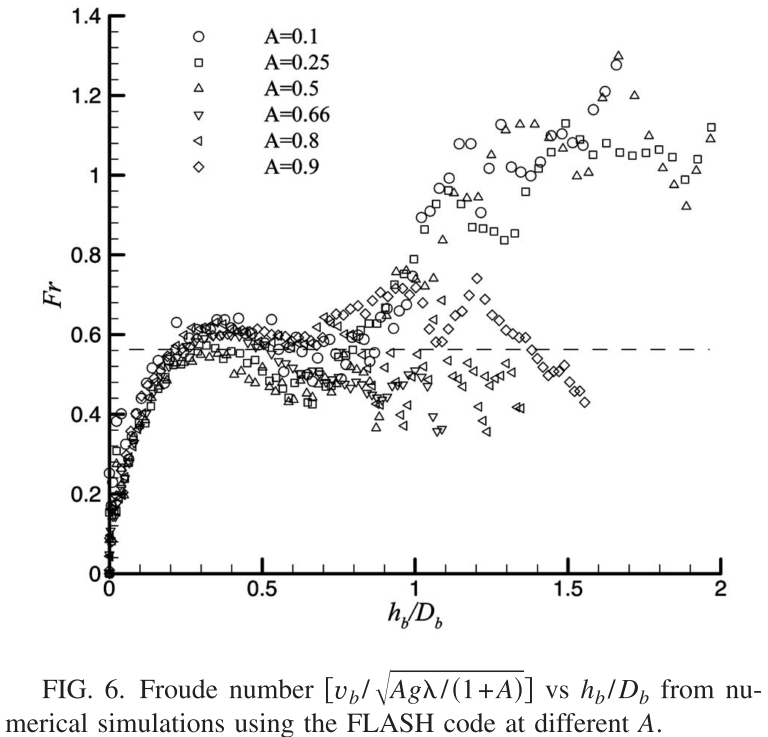
\includegraphics[height=0.5\textheight]{graphics/fr_flash.png}
~~~~
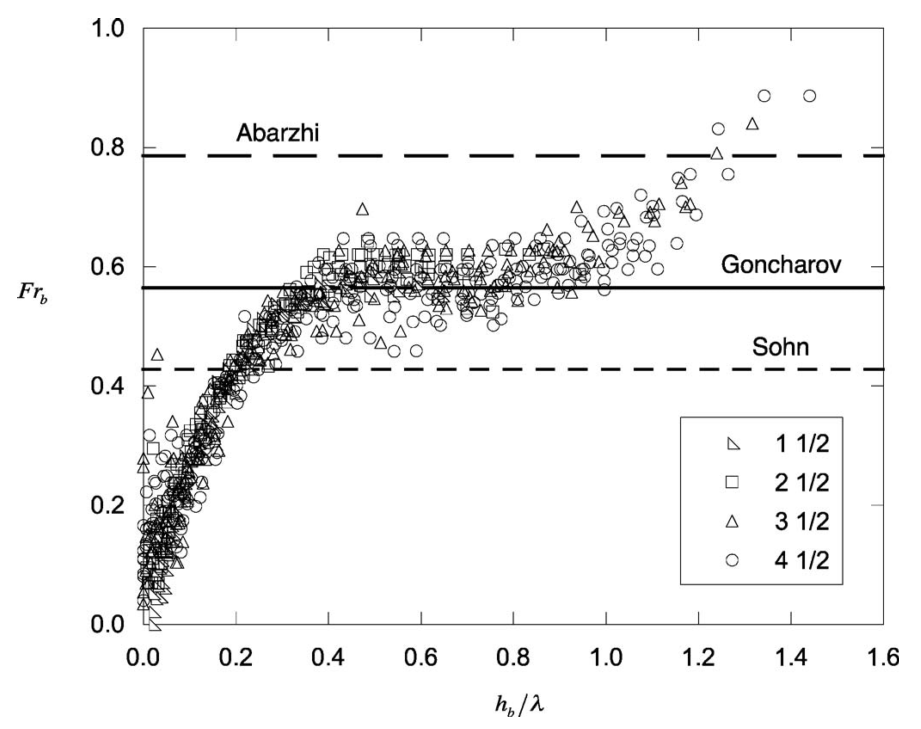
\includegraphics[height=0.5\textheight]{graphics/wilkinson_Fr.png}

{\footnotesize Simulations by Ramaprabhu and Dimonte, experiments by Wilkinson and Jacobs.}
}
\end{frame}

%===============================================================%
\section{Hypothesis}
%===============================================================%

\begin{frame}{Hypothesis: buoyancy-drag with ???}
Potential flow models assume no vorticity generation at the boundary,
which doesn't make sense for low-Atwood flows.

\vspace{20pt} \pause
Let's focus on buoyancy-drag instead:
\begin{equation*}
(\rho_1 + \rho_2) \mathcal{V} \ddot{h} = (\rho_2 - \rho_1) \mathcal{V} g - C \rho \dot{h}^2 \mathcal{A},
\end{equation*}
where $h$ is the bubble height, $\mathcal{V}, \mathcal{A}$ are characteristic volumes and areas, resp, and $C$ is a drag coefficient.

\vspace{20pt} \pause
For the single-mode RTI, $\mathcal{V} \sim \lambda^2 h$ and $\mathcal{A} \sim \lambda^2$, so:
\begin{equation*}
\dot{h}\left[\ddot{h} == 0\right] \sim \sqrt{h}
\end{equation*}
There is no terminal velocity at all!

\end{frame}


\begin{frame}{Hypothesis: buoyancy-drag with viscosity}
To balance the buoyancy, we add a viscous drag term:
\begin{equation*}
F_\nu \sim C \nu h \dot{h},
\end{equation*}
which is linear in $h$ so it can balance the buoyancy.
\begin{equation*}
\dot{h}\left[\ddot{h} == 0\right] = \frac{A g \lambda^2}{C \nu}
\end{equation*}
\pause

The growth is still terminal, but generally at a greater bubble velocity than predicted by inviscid potential flow models.
\vspace{20pt} \pause
\begin{exampleblock}{}
Let's build this idea into a full model.
\end{exampleblock}
\end{frame}

\begin{frame}
Write down the forces and inertias with undetermined coefficients.
\begin{align*}
\text{Force} &= \overbrace{C_0 A g \lambda^2 h}^{\text{buoyancy}} - \overbrace{C_1 \lambda^2 \dot{h}^2}^{\text{form drag}} - \overbrace{C_2 \nu h \dot{h}}^{\text{skin drag}} \\
\text{Inertia} &= \underbrace{C_3 \lambda^2 h}_{\text{cylinder}} + \underbrace{C_4 \lambda^3}_{\text{sphere}}
\end{align*}\pause

We can drop $C_0$ and simplify:
\begin{equation*}
\ddot{h} = \frac{A g h - C_1 \dot{h^2} - C_2 \nu (h/\lambda^2) \dot{h}}{C_3 h + C_4 \lambda}
\end{equation*}
which has an asymptotic terminal velocity:
\begin{equation*}
\dot{h} = \frac{A g \lambda^2}{C_2 \nu}
\end{equation*}\pause
This is a problem: mixing.
\end{frame}

\begin{frame}
If $\dot{h}$ is bounded, mixing ultimately dominates the inflow of pure fluid.
\begin{equation*}
\frac{d V_p}{dt} \sim \lambda^2 \dot{h} - D h 
\end{equation*}
\pause

We'll track the volume of mixed fluid instead, $V_m \equiv M$, and define the effective Atwood number wrt the volume fraction of mixed fluid:
\begin{equation*}
A = A_0 \left(1 - \frac{M}{V}\right)
\end{equation*}
where $A_0$ is the Atwood number of pure fluids.
\vspace{20pt} \pause

Now we need a model for $M$, but we can check it directly.
\end{frame}

\begin{frame}
Assume the bubble has two parallel diffusive planar interfaces:
\begin{equation*}
\phi_{1D}(r) \sim \text{erf}\left[\frac{r}{\delta}\right] - \text{erf}\left[\frac{r - d}{\delta}\right]
\end{equation*}
where $\phi_{1D}$ is the 1D mass profile, $\delta$ is the interface width, and $d$ is the bubble diameter.
\vspace{20pt}\pause

Integrating and multiplying by a surface area term:
\begin{equation*}
M \approx \overbrace{\left(C_5 \lambda h + C_6 \lambda^2\right)}^{\text{surface area}} \overbrace{\left[\frac{2 \delta}{\sqrt{\pi}} \left(1 - e^{-d^2 / \delta^2}\right) + 2 d \left(1 - \text{erf}\left[\frac{d}{\delta}\right]\right)\right]}^{\text{1D mixing}}
\end{equation*}
with $d = C_5 \lambda / 8$, $\delta = 2 \sqrt{D t}$, and a generic volume:
\begin{equation*}
V = C_7 \lambda^2 h + C_8 \lambda^3
\end{equation*}
\end{frame}

\begin{frame}
We can constrain 3 parameters by fitting limits:
\begin{itemize}
  \item $C_4 = (2 \pi)^{-1}$ from the inviscid immiscible linear theory
  \item $C_6 = 1$ from matching the initial condition
  \item $C_8 = \pi^{-1}$ from the miscible linear theory
\end{itemize}

We can estimate the rest by physical argument:
\begin{itemize}
  \item $C_1$ from known drag coefficients
  \item $C_2$ from Poiseuille flow
  \item $C_3, C_7$ should be about 1
  \item $C_5$ should be about $\pi$
\end{itemize}
\end{frame}

\begin{frame}
\textbf{Hypothesis:} this model captures the dynamics of the low-Atwood single-mode Rayleigh-Taylor instability in cases when the bubble has a steady structure, i.e. moderate Grashof number (square of Reynolds number).
\end{frame}

%===============================================================%
\section{Experiments}
%===============================================================%

\begin{frame}{Experiment 1: validation of simulations}
Experiments are \textit{hard}, but we might be able to use direct numerical simulations
 instead.
\begin{itemize}
  \item Method: very high order spectral elements
  \item Implementation: specially tailored version of Nek5000 (NekBox)
\end{itemize}
\vspace{20pt}\pause

Two important qualifications of the simulations:
\begin{enumerate}
  \item Do they include all relevant physical processes?
  \item Are they accurate and cheap enough to do a parameter sweep?
\end{enumerate}
\end{frame}

\begin{frame}{Comparison to Wilkinson and Jacobs}
The most direct validation is to replicate the re-acceleration-originating experiment of Wilkinson and Jacobs.

\begin{block}{Three approximations}
\begin{itemize}
  \item Boussinesq approximation at $A = 0.15$
  \item Unit order Schmidt number, $\text{Sc} = \{1,3.5,7\}$
  \item Stationary ($u = 0$) initial condition
\end{itemize}
\end{block}

\begin{exampleblock}{}
Will the simulations agree quantitatively?
\end{exampleblock}
\end{frame}

\begin{frame}{Validation results}
\begin{center}
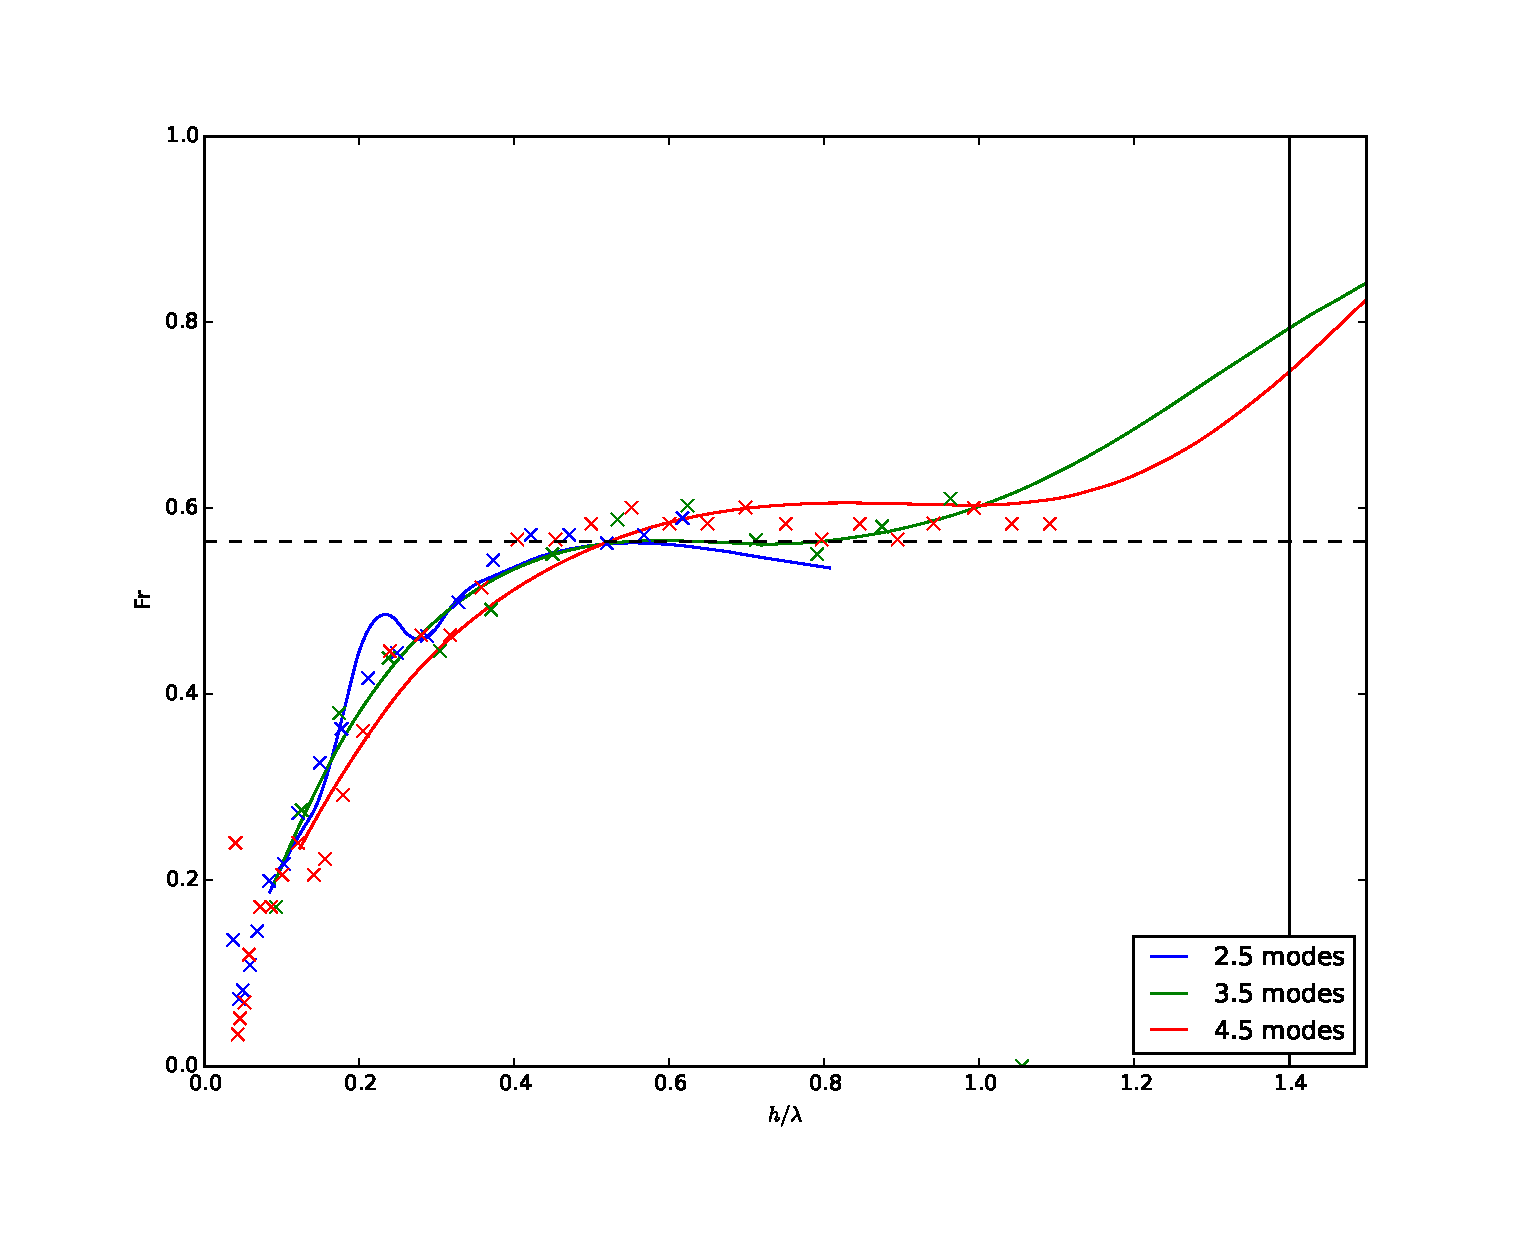
\includegraphics[height=0.9\textheight]{graphics/Fr.eps}
\end{center}
\end{frame}

\begin{frame}{Convergence and performance}
\begin{center}
\vspace{-10pt}
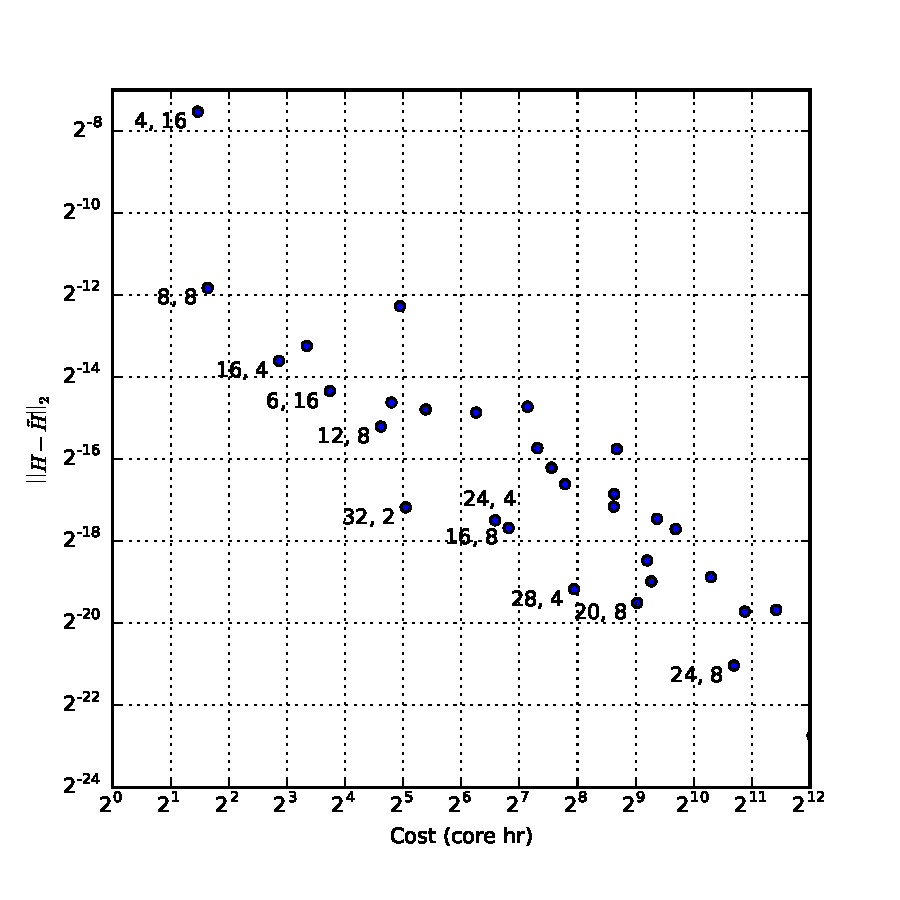
\includegraphics[height=0.89\textheight]{graphics/mira_H.pdf}
\end{center}
\vspace{-20pt}
Selected discretization with error in height below $10^{-4}$
\end{frame}


\begin{frame}{Dataset generation}
Sampled Grashof from $\left[10^2,10^6\right]$ and Schmidt from $\left[1,64\right]$.
\begin{itemize}
  \item 28 distinct simulations
\end{itemize}
\vspace{10pt} \pause

Most accurate dataset available:
\begin{itemize}
  \item Relative error in bubble height less than $0.01\%$
  \item Domain height of $22\lambda$ (vs $6\lambda$)
\end{itemize}
\vspace{10pt} \pause

Flow simulated until either:
\begin{itemize}
  \item Bubble stops rising (complete)
  \item Bubble reaches $3/4$ domain height (incomplete)
\end{itemize}
\end{frame}

\begin{frame}
The 1-parameter mixing model is fit first, using the true bubble height as input.
\begin{itemize}
  \item Prevents over-fitting
  \item Non-linear fit with basin-hopping/sequential-least-squares
\end{itemize}
\vspace{20pt} \pause

The 4-parameter dynamics model is fit given the mixing model.
\begin{itemize}
  \item Non-linear fit with covariance matrix assisted evolution strategy
  \item L2 (Tinkhonov) regularization about coefficient estimates
  \item Constraints set by physical argument, e.g. $C_3 \ge 1$.
  \item Polished with sequential-least-squares
\end{itemize}
\end{frame}

%===============================================================%
\section{Results}
%===============================================================%
\begin{frame}[c]{Results: Fit trajectories}
The following slides will contain plots of non-dimensional:
\begin{itemize}
  \item Bubble height $H / \lambda$
  \item Bubble velocity (Froude number): $v / \sqrt{A g \lambda}$
  \item Mixed volume: $M / \lambda^3$
\end{itemize}
versus time for a few representative trajectories.
\end{frame}

\begin{frame}[plain]
\begin{columns}[c]
\column{0.5\textwidth}
\begin{itemize}
  \item $\text{Gr} = 4.3 \times 10^4$
  \item $\text{Sc} = 8$
  \item $\text{Ra} = 3.5 \times 10^5$
  \item $C_1 = 0.30$
  \item $C_2 = 161.1$
  \item $C_3 = 1.00$
  \item $C_5 = 3.86$
  \item $C_7 = 2.49$
  \item $||H-h||_2/H = 0.29\%$
  \item $||M-m||_2/M = 0.24\%$
\end{itemize}
\column{0.5\textwidth}
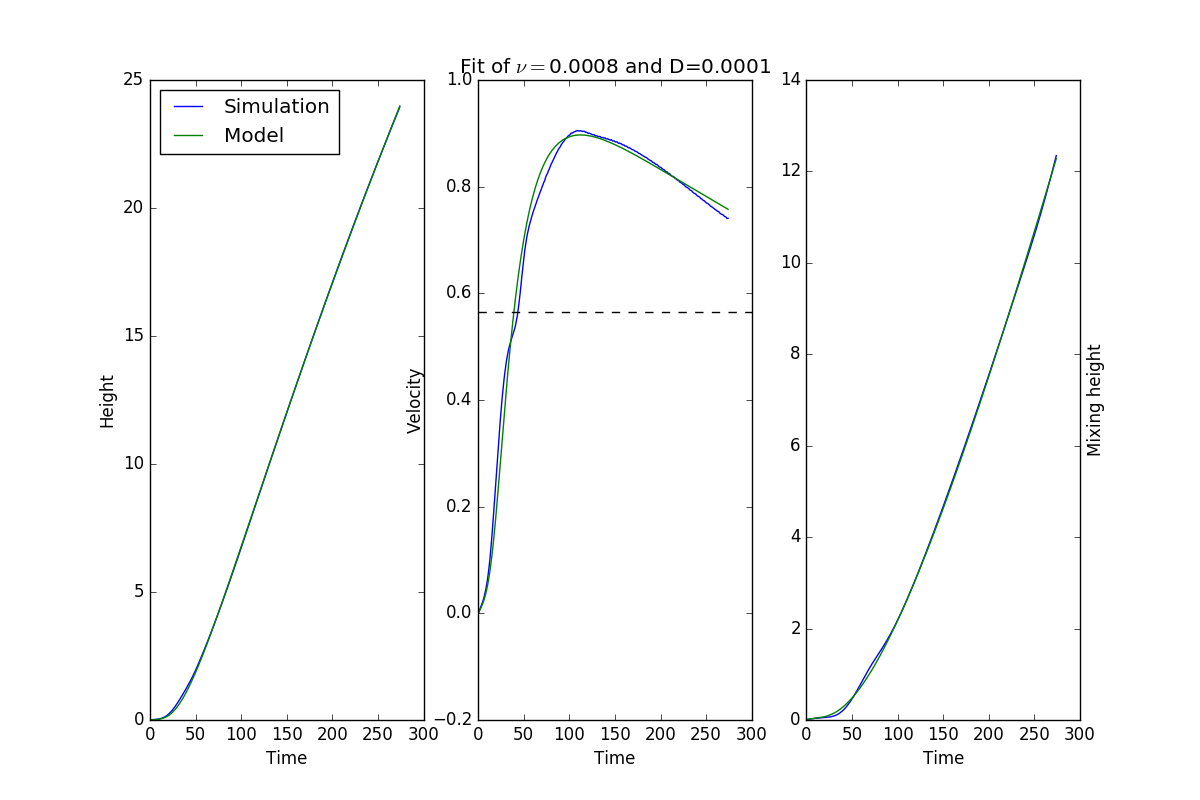
\includegraphics[height=1.05\textheight]{graphics/H-8-1.png}
\end{columns}
\end{frame}



\begin{frame}[plain]
\begin{columns}[c]
\column{0.5\textwidth}
\begin{itemize}
  \item $\text{Gr} = 6.9 \times 10^5$
  \item $\text{Sc} = 2$
  \item $\text{Ra} = 1.4 \times 10^6$
  \item $C_1 = 0.46$
  \item $C_2 = 136.3$
  \item $C_3 = 1.00$
  \item $C_5 = 3.18$
  \item $C_7 = 1.05$
  \item $||H-h||_2/H = 0.74\%$
  \item $||M-m||_2/M = 2.04\%$
\end{itemize}
\column{0.5\textwidth}
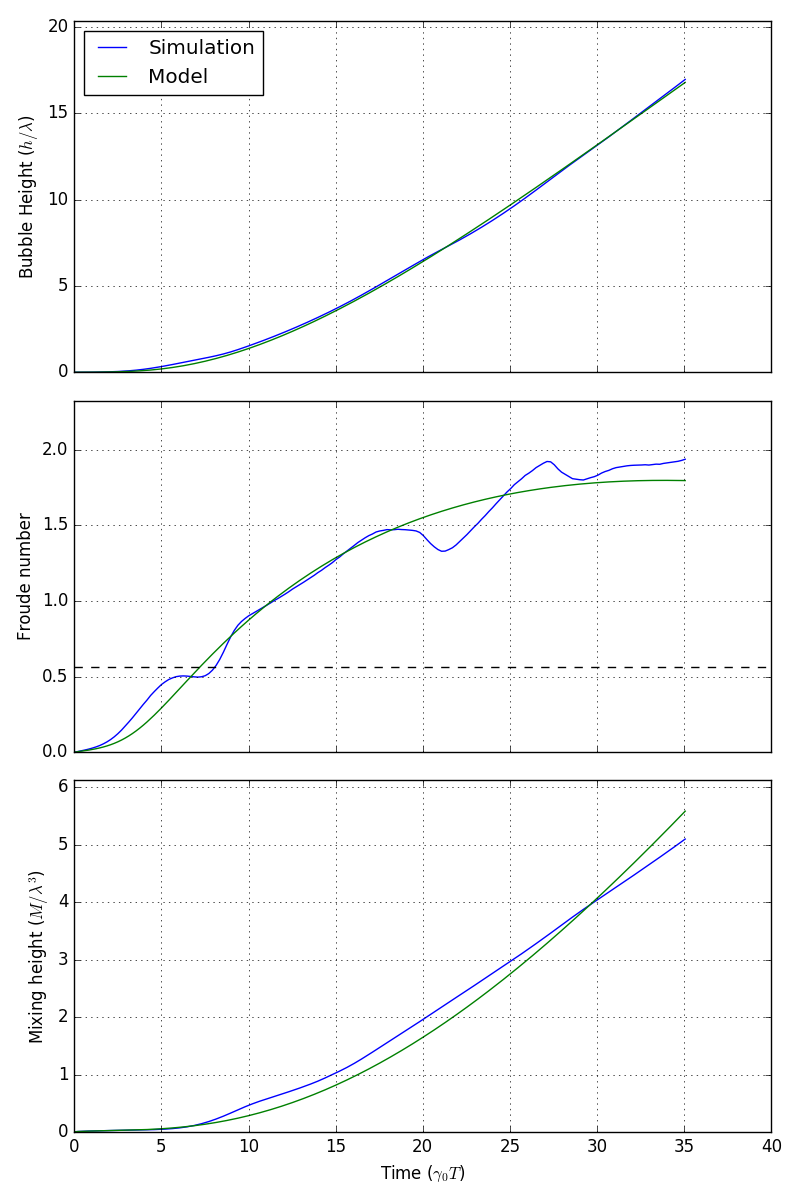
\includegraphics[height=1.05\textheight]{graphics/H-2-1.png}
\end{columns}
\end{frame}

\begin{frame}[plain]
\begin{columns}[c]
\column{0.5\textwidth}
\begin{itemize}
  \item $\text{Gr} = 4.3 \times 10^4$
  \item $\text{Sc} = 1$
  \item $\text{Ra} = 4.3 \times 10^4$
  \item $C_1 = 0.00$
  \item $C_2 = 96.5$
  \item $C_3 = 1.54$
  \item $C_5 = 2.27$
  \item $C_7 = 1.02$
  \item $||H-h||_2/H = 0.14\%$
  \item $||M-m||_2/M = 1.22\%$
\end{itemize}
\column{0.5\textwidth}
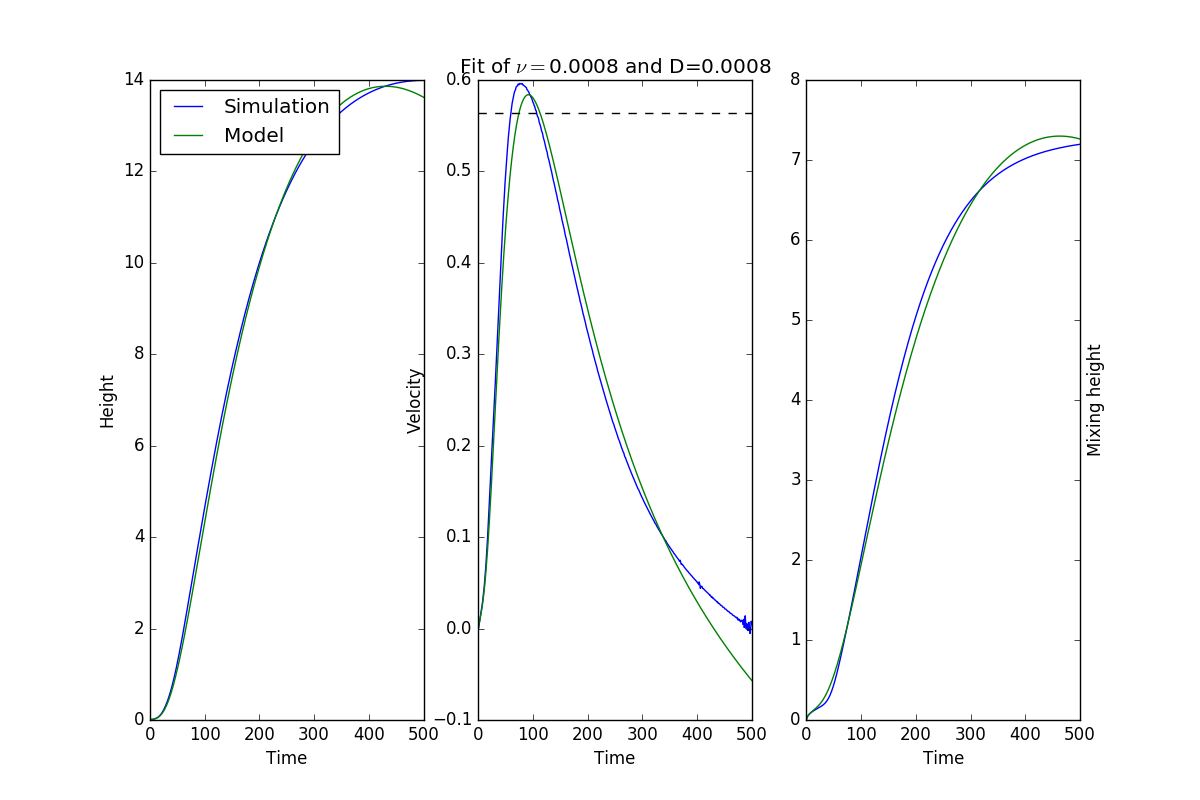
\includegraphics[height=1.05\textheight]{graphics/H-8-8.png}
\end{columns}
\end{frame}

\begin{frame}[plain]
\begin{columns}[c]
\column{0.5\textwidth}
\begin{itemize}
  \item $\text{Gr} = 6.8 \times 10^2$
  \item $\text{Sc} = 16$
  \item $\text{Ra} = 1.1 \times 10^4$
  \item $C_1 = 0.00$
  \item $C_2 = 69.5$
  \item $C_3 = 9.10$
  \item $C_5 = 2.47$
  \item $C_7 = 1.00$
  \item $||H-h||_2/H = 0.22\%$
  \item $||M-m||_2/M = 0.95\%$
\end{itemize}
\column{0.5\textwidth}
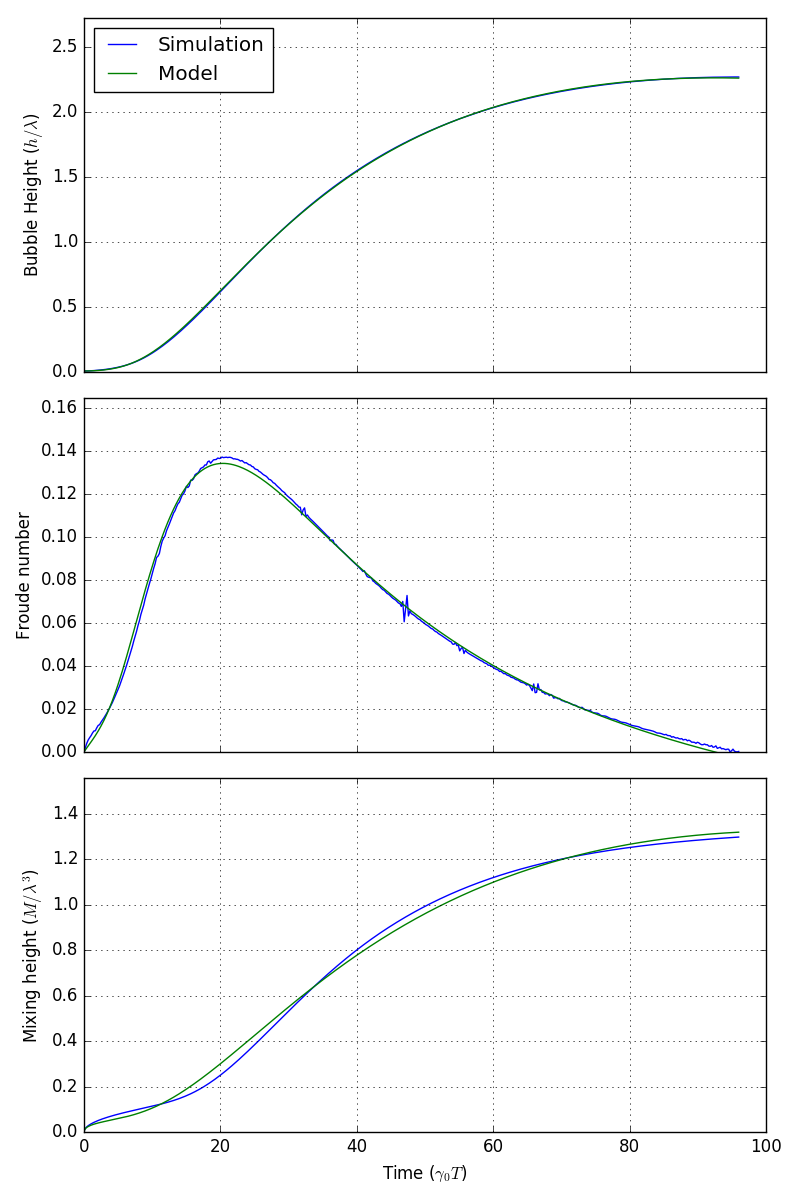
\includegraphics[height=1.05\textheight]{graphics/H-64-4.png}
\end{columns}
\end{frame}





\begin{frame}[t]{Coefficients wrt Rayleigh and Schmidt}
%A quick review:
%\begin{equation*}
%\text{Gr} = \frac{A g \lambda^3}{\nu^2} \qquad \text{Sc} = \frac{\nu}{D} \qquad \text{Ra} = \text{Gr} \text{Sc} = \frac{A g \lambda^3}{\nu D}
%\end{equation*}

At early times, we can ignore viscosity and diffusion:
\begin{equation*}
\tau \sim \sqrt{\frac{\lambda}{A g}} \qquad \tilde{v} \sim \sqrt{A g \lambda}
\end{equation*}

At moderate times, viscosity becomes important
\begin{equation*}
\tau_\nu \sim \frac{\nu}{A g \lambda} \qquad \tilde{v} \sim \frac{A g \lambda^2}{\nu} \qquad \frac{\delta}{\lambda} \sim \sqrt{\frac{D \tau}{\lambda^2}} = \sqrt{\frac{1}{\text{Ra}}}
\end{equation*}

At late times, diffusion dominates
\begin{equation*}
\tau_D \sim \frac{\lambda^2}{D} \qquad \tilde{v} \sim \frac{A g \lambda^2}{\nu} \qquad \frac{h}{\lambda} \sim \frac{\tilde{v} \tau_D}{\lambda} = \text{Ra}
\end{equation*}
\end{frame}

\begin{frame}[t]{Relative error in bubble height}
\begin{center}
\vspace{-11pt}
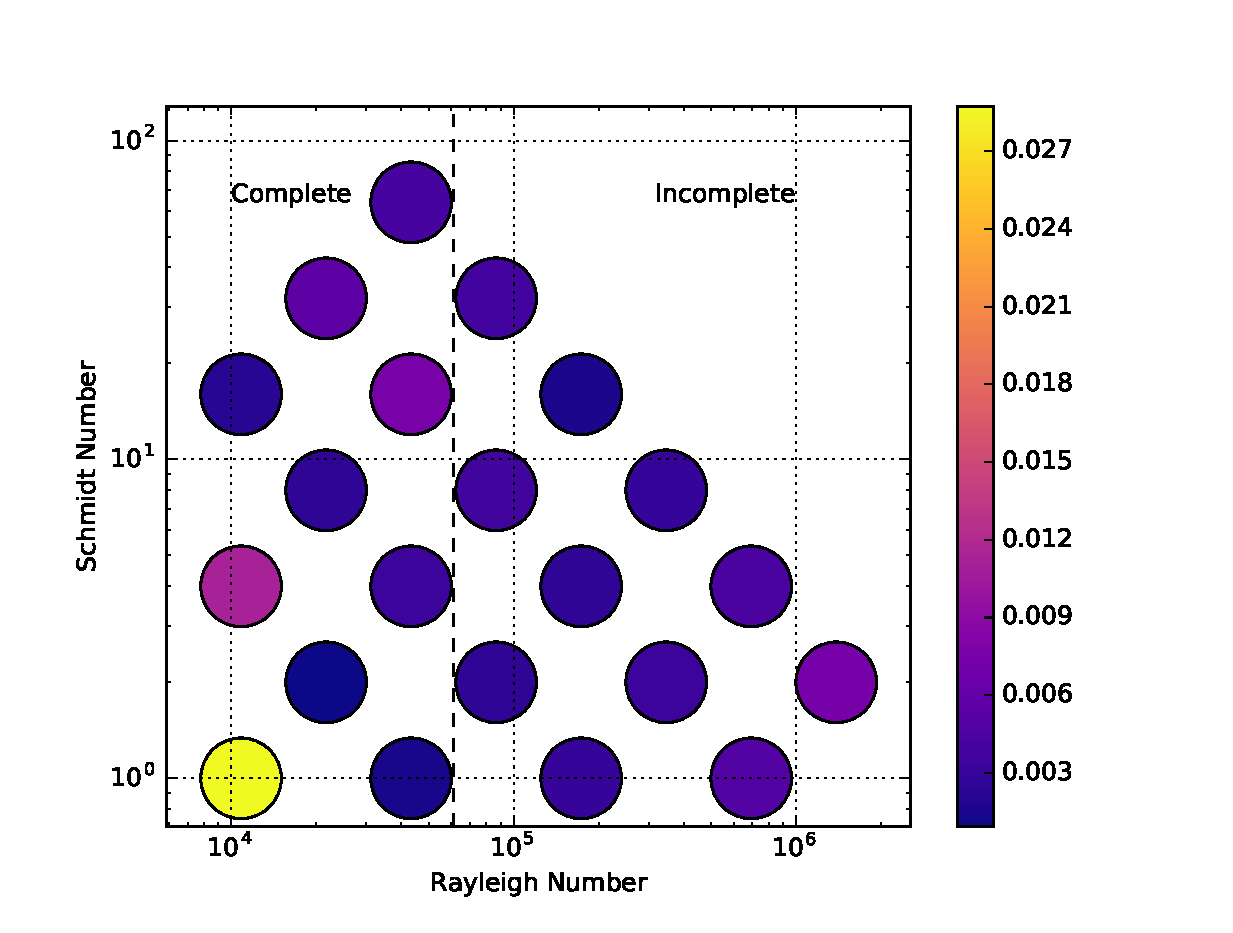
\includegraphics[width=0.85\textwidth]{graphics/DynamicsError-vs-Rayleigh-Schmidt.eps}
\end{center}
\end{frame}

\begin{frame}[t]{Relative error in mixed volume}
\begin{center}
\vspace{-11pt}
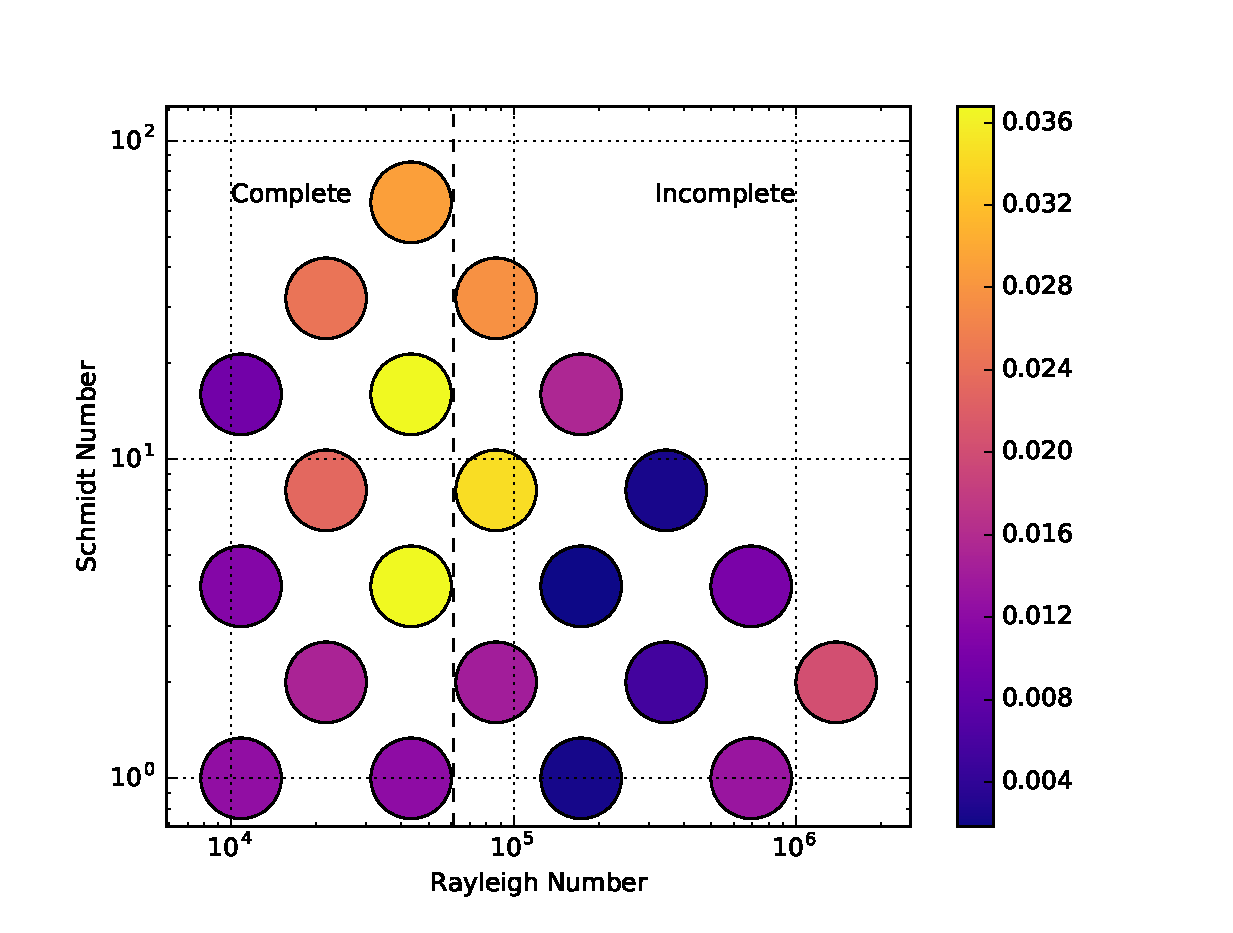
\includegraphics[width=0.85\textwidth]{graphics/MixingError-vs-Rayleigh-Schmidt.eps}
\end{center}
\end{frame}



\begin{frame}[t]{$C_1$ (drag coefficient)}
\begin{center}
\vspace{-11pt}
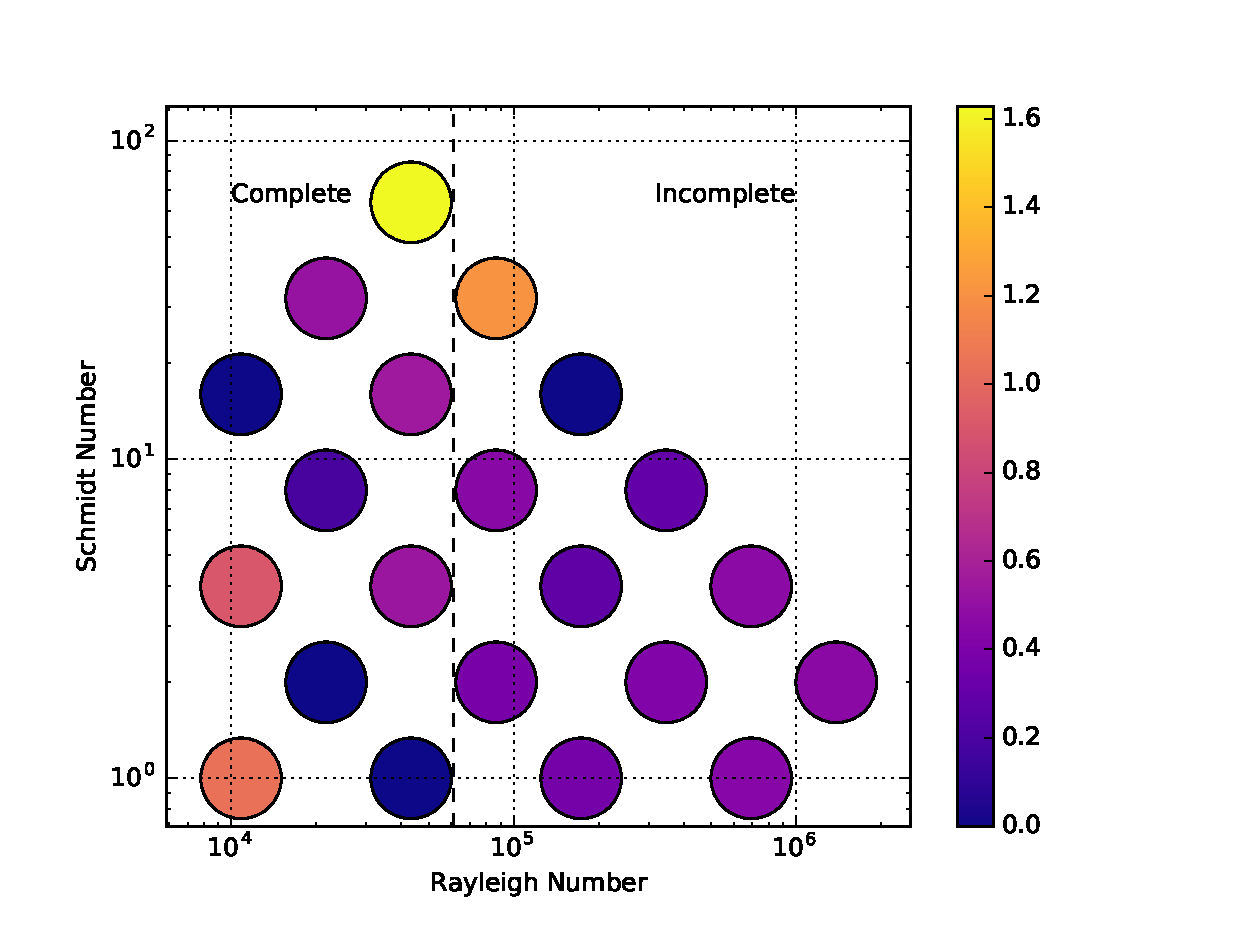
\includegraphics[width=0.85\textwidth]{graphics/C1-vs-Rayleigh-Schmidt.eps}
\end{center}
\end{frame}

\begin{frame}[t]{$C_2$ (friction factor)}
\begin{center}
\vspace{-11pt}
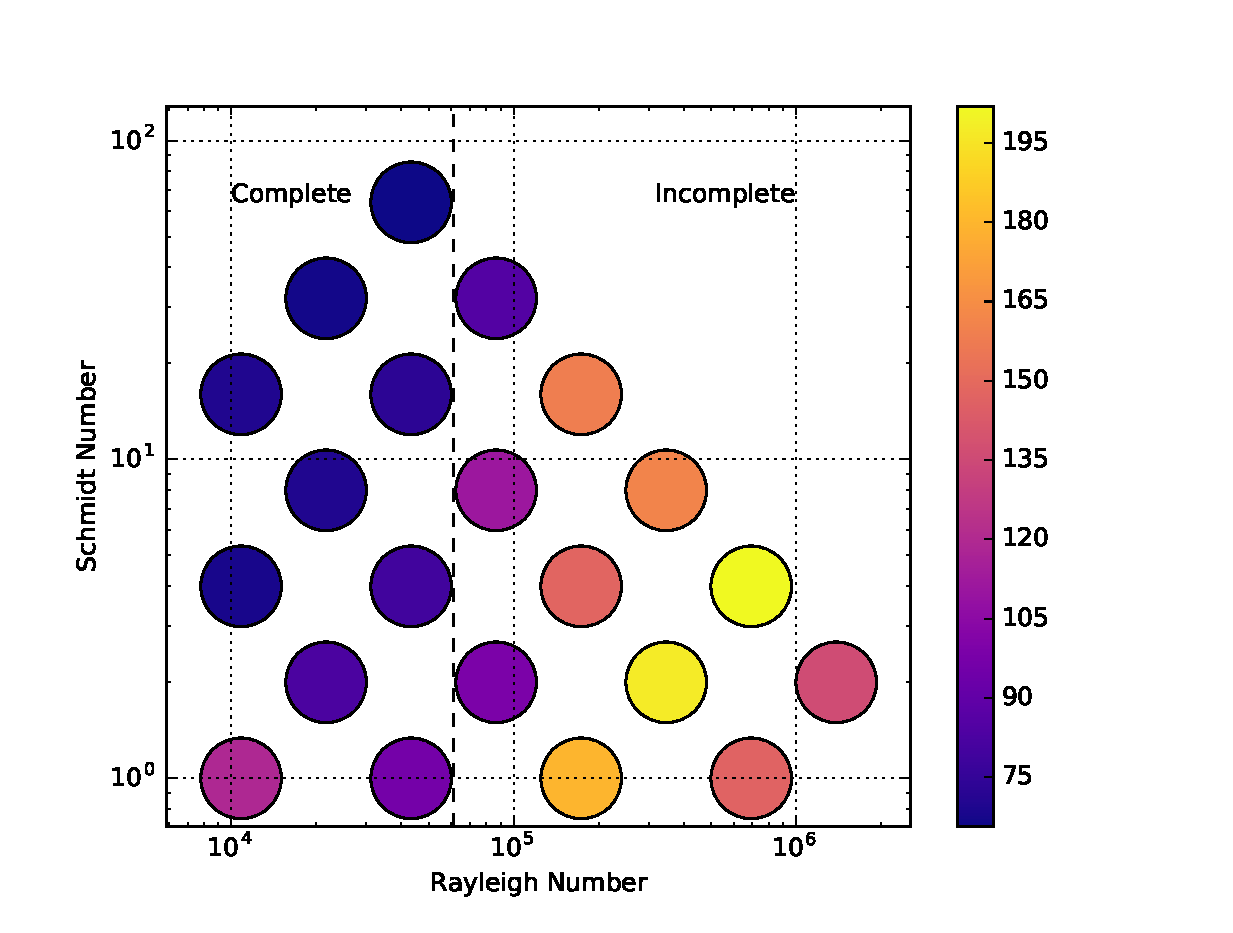
\includegraphics[width=0.85\textwidth]{graphics/C2-vs-Rayleigh-Schmidt.eps}
\end{center}
\end{frame}

\begin{frame}[t]{$C_3$ (inertial ratio)}
\begin{center}
\vspace{-11pt}
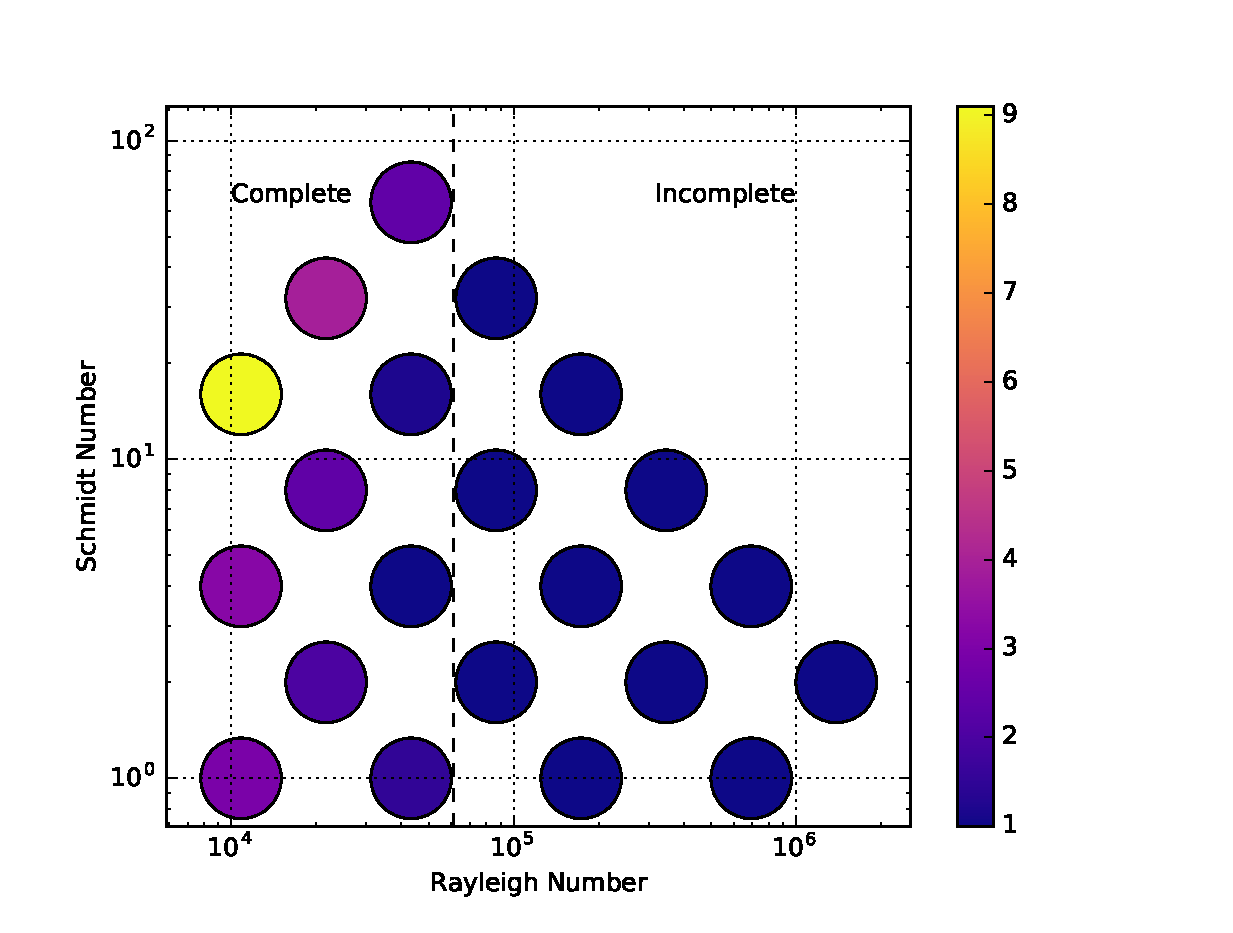
\includegraphics[width=0.85\textwidth]{graphics/C3-vs-Rayleigh-Schmidt.eps}
\end{center}
\end{frame}

\begin{frame}[t]{$C_5$ (mixing area)}
\begin{center}
\vspace{-11pt}
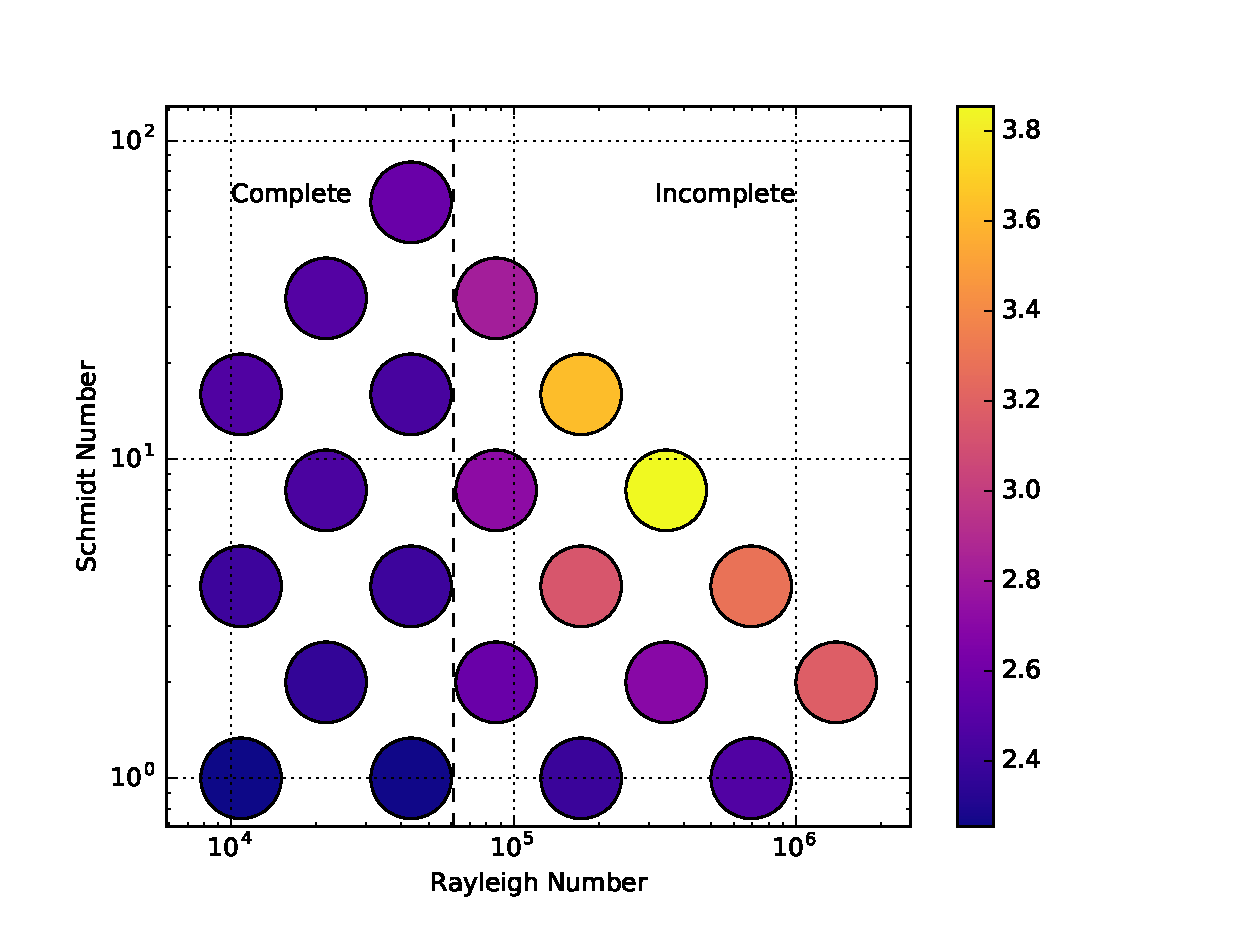
\includegraphics[width=0.85\textwidth]{graphics/C5-vs-Rayleigh-Schmidt.eps}
\end{center}
\end{frame}

\begin{frame}[t]{$C_7$ (mixing ratio)}
\begin{center}
\vspace{-11pt}
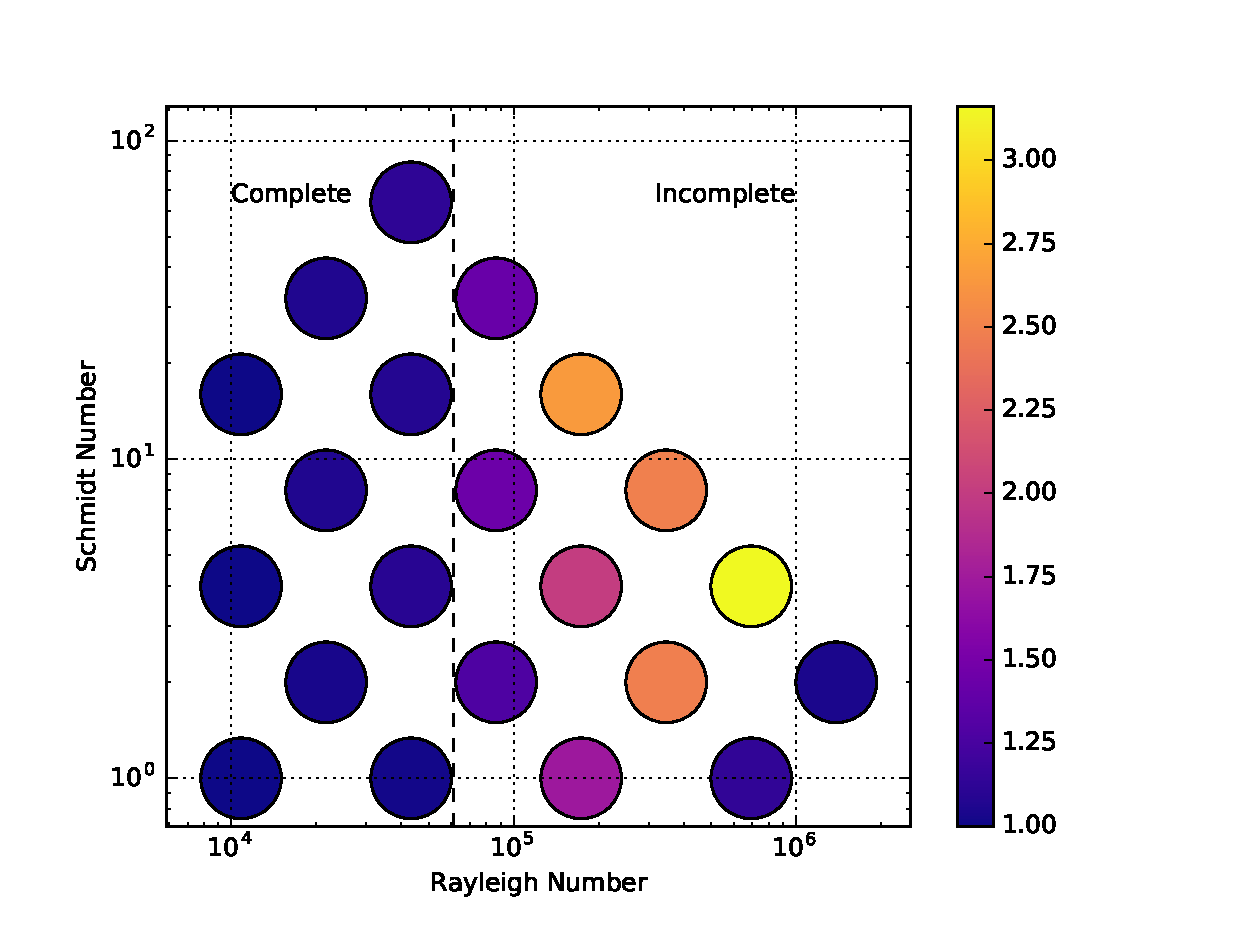
\includegraphics[width=0.85\textwidth]{graphics/C7-vs-Rayleigh-Schmidt.eps}
\end{center}
\end{frame}

%===============================================================%
\section{Conclusions}
%===============================================================%
\begin{frame}{Methodology}
Direct numerical simulations are effective proxies for experiments
\begin{itemize}
  \item Boussinesq, low-Schmidt, and incompressible approximations valid for low-Atwood RTI
  \item Simulation state of the art is capable of $\text{Ra} = 4 \times 10^{4}$
\end{itemize}
\vspace{10pt} \pause

Buoyancy-drag models can be fit with CMA-ES $+$ regularization
\begin{itemize}
  \item Fits coefficients consistently
  \item Reaches error rates $\sim 0.1 \%$
\end{itemize}
\end{frame}

\begin{frame}{Modeling}
The proposed model is quantitatively descriptive
\begin{itemize}
  \item Depends only on initial conditions
  \item Low error rates over a range of Grashof and Schmidt numbers
  \item Admits physical interpretation of parameters
\end{itemize}

Three coefficients have simple behavior
\begin{itemize}
  \item $C_3, C_7$ ratios are nearly $1$
  \item $C_2$ increases with the Grashof number
\end{itemize}

Two coefficients have complex behavior
\begin{itemize}
  \item $C_1$ is mostly $\approx 0.5$, but has many outliers
  \item $C_5$ decreases with diffusivity, but has a peak in Grashof
\end{itemize}
\end{frame}

\begin{frame}{Flow physics}
Dissipation dominates the late-time behavior
\begin{itemize}
  \item The only late-time velocity is viscous
  \item Any finite viscosity and diffusivity results in mixing death
\end{itemize}

\textit{Re-acceleration} is (just) a moderate-time transient
\begin{itemize}
  \item This model misses re-acceleration but gets the later flow right
  \item There is likely a missing term in the model
  \item The vortex ring at the bubble tip is a prime suspect
\end{itemize}
\end{frame}

\appendix
%===============================================================%
\section*{Backup slides}
%===============================================================%
\begin{frame}{Backup slide}

	Some stuff here.

%\resizebox{\textwidth}{!}{
\tikzstyle{block} = [rectangle, draw, 
    text width=10em, text centered, rounded corners, minimum height=10em]
\tikzstyle{intro} = [block, fill=blue!20]  
\tikzstyle{model} = [block, fill=yellow!20] 
\tikzstyle{valid} = [block, fill=black!30!green] 
\tikzstyle{optim} = [block, fill=black!50!green] 
\tikzstyle{other} = [block, fill=black!10!purple] 
\tikzstyle{sloud} = [draw, star,fill=green!20, minimum height=2em]
\tikzstyle{ar}    = [->, thick, shorten <=8pt, shorten >=8pt]
\tikzstyle{wlock} = [rectangle, draw, 
    text width=5em, text centered, minimum height=4em]


\begin{tikzpicture}[node distance=5cm, auto]
\node[intro] (layzer) {Potential flow models of Layzer and Goncharov};
\node[intro, right of=layzer] (wilk) {Single mode experiments by Wilkinson};
\node[model, right of=wilk] (bdm) {Buoyancy-drag model with viscosity};
\node[model, right of=bdm, node distance=8cm] (param) {Model parameters and accuracy};
\node[model, right of=param] (behavior) {Model behavior};
\node[model, right of=behavior] (ques) {Open questions};

\node[valid, below of=bdm, node distance=8cm] (val) {Validation against Wilkinson's experiments};
\node[valid, left of=val] (sim) {Simulation with spectral element method};
\node[valid, left of=sim] (NS) {Incompressible Navier-Stokes};
\node[optim, right of=val] (conv) {Convergence \& performance study};
\node[optim, right of=conv] (tuning) {Tuning for efficiency};
\node[optim, right of=tuning] (data) {Simulation of data set};

\node[other, below of=sim] (ts) {Mixed order time-steppers};
\node[other, below of=tuning] (xsmm) {LIBXSMM etc.};
\node[other, below of=data] (dask) {DAG-based workflows in nekpy with dask};
\node[other, below of=conv] (proj) {Subspace projection for successive RHS};

\path (layzer) edge[ar] (wilk);
\path (wilk) edge[ar] (bdm);
\path (bdm) edge[ar, dotted] node {Hard analytically} (param);
\path (param) edge[ar] (behavior);
\path (behavior) edge[ar] (ques);

\path (NS) edge[ar] (sim);
\path (sim) edge[ar] (val);
\path (val) edge[ar] (conv);
\path (conv) edge[ar] (tuning);
\path (tuning) edge[ar] (data);

\path (bdm) edge[ar, out=270, in=90] (NS);
\path (data) edge[ar, out=90, in=270] (param);

\path (ts) edge[ar, dotted] (sim);
\path (xsmm) edge[ar, dotted] (tuning);
\path (dask) edge[ar, dotted] (data);
\path (proj) edge[ar, dotted] (conv);

%\path () edge[ar] ();
%\path () edge[ar] ();

%\path (ibc) edge[ar, bend right=45] (pet);
%\path (inp) edge[ar, bend right=45] (pet);
%\path (raw) edge[ar, bend left=45] (pet);
%\path (opp) edge[ar, bend left=45] (pet);

\end{tikzpicture}
}
\end{frame}

%===============================================================% 
\end{document}
%===============================================================%
